% classes
\documentclass{article}

% packages
\usepackage{graphicx}
\usepackage{fancyhdr} % Required for custom headers
\usepackage{lastpage} % Required to determine the last page for the footer
\usepackage{extramarks} % Required for headers and footers
\usepackage{courier} % Required for the courier font

\usepackage{color}
\usepackage{enumitem}

\usepackage{hyperref}


% page layout


\topmargin=-0.45in
\evensidemargin=0in
\oddsidemargin=0in

\textwidth=6.5in
\textheight=9.0in

\headsep=0.25in

\linespread{1.1} % Line spacing
 
\pagestyle{fancy}

% headers and footers

\fancyhf{}

\lhead{INTR 100 Breaking Intuition}

\rhead{
\includegraphics[width=0.045\textwidth]{wmlogo.jpg}}



% document body

\begin{document}

\vspace*{.01mm}

\begin{center}

\Large{\textcolor{blue}{\textbf{Lab 5.}  Reimagining New York City}}

\vspace{4mm}

\textit{Due by noon on Friday, November 13th}\\

\end{center}

\begin{figure}[h!]
\begin{center}
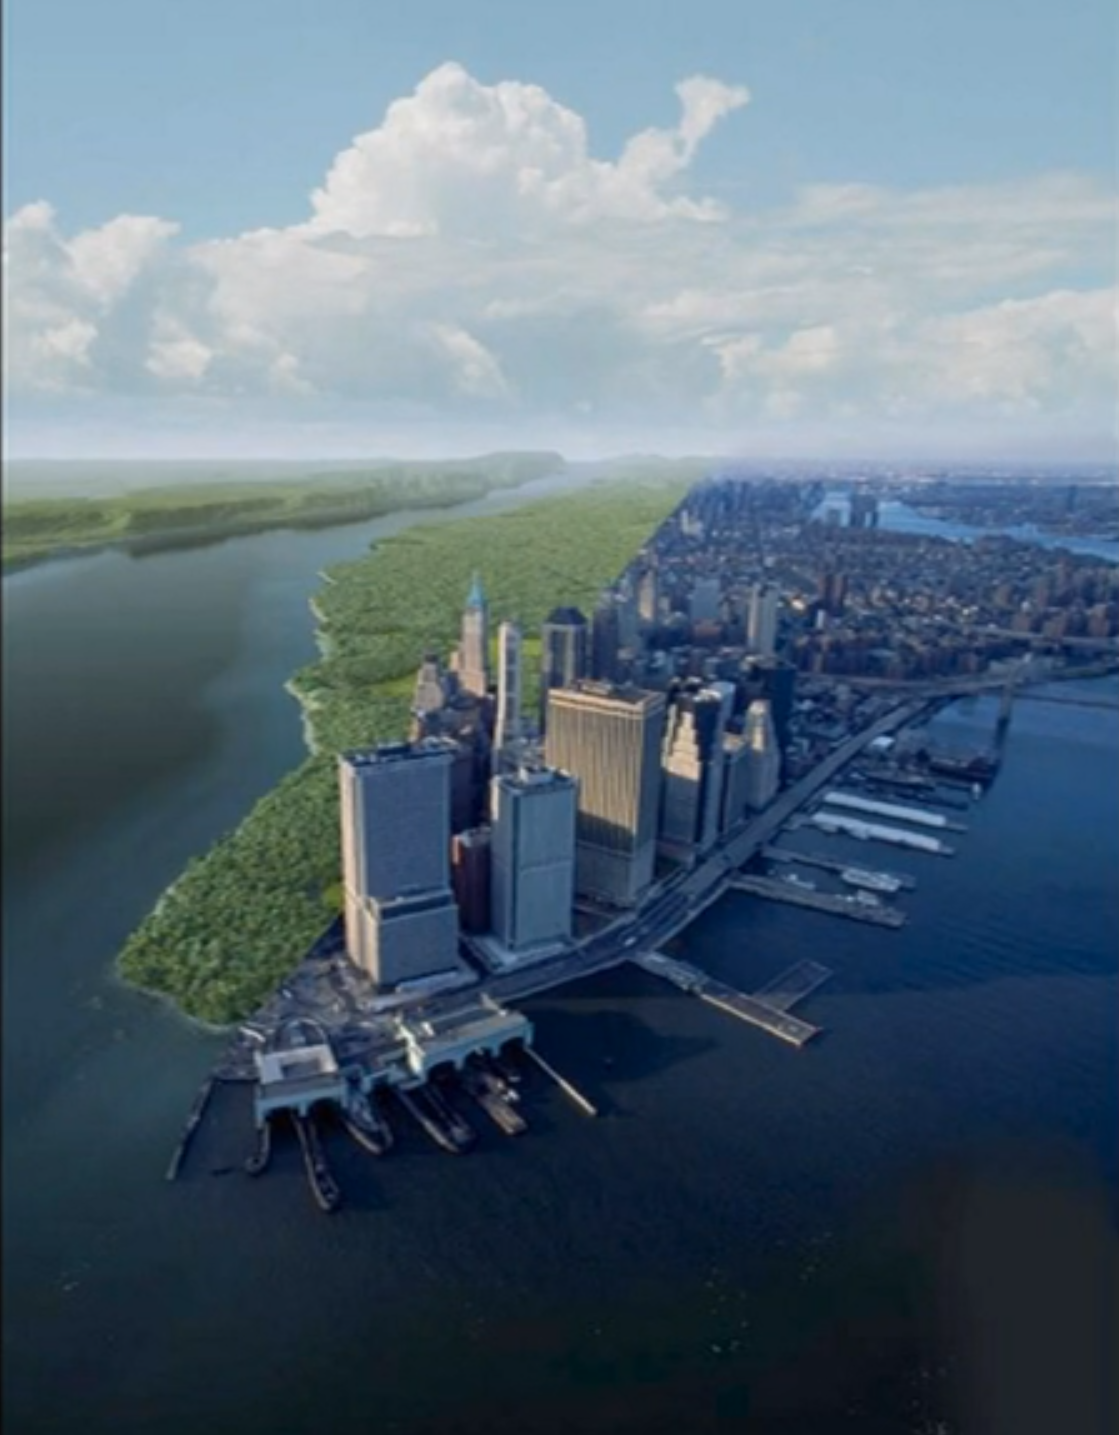
\includegraphics[width=0.75\textwidth]{nyc.png}

\end{center}
\end{figure}

\setlength{\parindent}{0cm}

\large{\textit{"And as the moon rose higher the inessential houses began to melt away until gradually I became aware of the old island here that flowered once for Dutch sailors' eyes - a fresh, green breast of the new world."}
\begin{flushright}
from Chapter 9 of F. Scott Fitzgerald's, The Great Gatsby
\end{flushright}
}


\newpage

% Enumerate the Laboratory Objectives

\large{\textbf{Laboratory in Brief:}}

\vspace{4mm}

\setlength{\leftskip}{1cm}

\setlength{\parindent}{0cm}

The purpose of this laboratory is to use the online land use planning tool Visionmaker to create a potential future for a neighborhood located somewhere in New York City.  First, you will choose a place in New York City, consider that place's natural habitat in 1609 and compare it to its existing condition in 2010.  Next, you will use Visionmaker  to reimagine transforming the existing state of your chosen place three times with an emphasis on economic, social and environmental values.  Finally, you will create a hypothetical vision for your neighborhood that optimizes environmental performance while also taking into consideration constraints for population growth and build out cost.

\vspace{4mm}

\setlength{\leftskip}{0cm}

\large{\textbf{Goals of this Laboratory:}}

\begin{enumerate}[leftmargin=15mm]

\item To choose a neighbourhood in New York City and reimagine it based on three different scenarios, each one emphasising economic, social or environmental values.

\item To reimagine that same neighbourhood while optimising environmental performance while also taking into consideration population and cost constraints.

\item To create a document that describes the vision for the chosen neighbourhood.

\end{enumerate}

% Enumerate the Laboratory Resources Needed

\large{\textbf{Software and Resources you will need or will be helpful:}}

\begin{enumerate}[leftmargin=15mm]

\item Watch Eric Sanderson's June 2009 TED talk: New York - before the City \\  
\url{http://www.ted.com/talks/eric_sanderson_pictures_new_york_before_the_city}

\item Goto to the New York City Vision maker website, create an account and login.  The website may have compatibility issues with some web browsers; use Firefox or Google Chrome if you experience problems. \\ 
\url{https://visionmaker.us/nyc/}

\item Additionally and as time permits, review material available at the project website, including relevant publications \\ 
\url{https://welikia.org}

\end{enumerate}

% Enumerate the Laboratory Objectives

\large{\textbf{Step by Step Instructions:}}

\begin{enumerate}[leftmargin=15mm]

\item Once you have created your account and logged into the Visionmaker portal, choose \textbf{Create New Vision} and set up your new vision by giving it a name.  Under the \textbf{Base on} selection button, choose \textbf{New York City (2014)} as the basis for your new vision.  After creating your new vision, you will want to start by choosing a neighbourhood somewhere in New York City.  If you are familiar with New York City, then this will be easy.  If you are not familiar with New York City, then try to think of a famous place that comes to your mind.  Following are some suggested locations.

\begin{itemize}

\item Times Square
\item The Empire State Building
\item The Brooklyn Bridge
\item Central Park
\item Broadway
\item Wall Street
\item Yankee Stadium
\item Harlem
\item Rockefeller Center
\item Madison Square Garden
\item JFK Airport

\end{itemize}

Once you have chosen your neighbourhood, find it in the Visionmaker portal and zoom in towards that location.  On the right hand side of the Visionmaker portal is the \textbf{zoom tool}, use it to bring your neighbourhood into focus at \textbf{zoom level 17}.  Explore and become familiar with your neighbourhood.

\item Once you have zoomed into your neighbourhood, click on the \textbf{Specify Vision Extent} tool from the toolbar on the right side of the portal interface.  Once the tool has been activated, blocks of land will highlight as the cursor traverses the aerial photograph of your New York City neighbourhood.  Use the \textbf{Specify Vision Extent} to select several continuous blocks of parcels.  Starting out by choosing eight to twelve continuous blocks of land should be good.  Once you have selected the blocks of land that will comprise your neighborhood, click on the \textbf{Save} button on the top middle of the portal.

\item After you have saved the \textbf{Vision Extent}, your neighbourhood will be transformed into individual pixels that represent the land use for that location.  See the Ecosystem Tool Key at the end of this document to review the colors representing various Built and Natural Environment land uses.  Select the \textbf{Grid Inspector Tool} and choose several of the grid cells within your neighborhood.  Note the existing land use designations as well as the natural habitat for several grid cells.  Then find the \textbf{Lifestyle/Climate Selectors} toolbar and choose the lifestyle of the average person who will inhabit your neighborhood.  Next find the \textbf{Environmental Performance toolbar} and choose the \textbf{Calculate button} to measure your neighborhood's environmental performance in terms of water, carbon, biodiversity, population and economics.  Click on the \textbf{Inputs \& Outputs bar} and also review these indicators.

\item For your first excercise, have fun trying to be Donald Trump! Transform each grid cell in your neighborhood into its highest and best economic use.  Transform low density residential uses to high density residential or commercial uses.  Increase the number of stories of mixed use retail and office buildings and introduce hotels (maximum number of floors is 999 although the tallest building in the world is only 160 stories).  Convert controlled access highways and freeways to parking decks, local streets and pedestrian pathways.  Add powerplants and water treatment facilities if you feel those are necessary or simply leave them external to your neighborhood vision.  Try to be realistic while also profit seeking.

Once you are finished, \textbf{recalculate the environmental performance} of your neighborhood and export the results.  Write two or three paragraphs describing your Donald Trump scenario, describing the absurdity of the amount of CO2 emitted and water consumed.  Compare your daytime and/or nighttime population density to another location somewhere on planet earth.  Likewise compare the construction and demolition costs to the GDP of one or more small countries.

\item Next imagine you are John Muir \& Jane Jacobs and transform your neighborhood by optimising environmental and social values.  Convert high density residential and commercial uses to single family homes or neighborhood restaurants.  Introduce forests, orchards, public parks or community recreational facilities.  Introduce universities or public meeting spaces and reduce the functional classification of transportation facilities, introduce pedestrian pathways and other open or common spaces.  Try to reduce carbon emissions, while maximizing species and habitat biodiversity while maintaining population or permitting it to increase.  

Once you are finished, recalculate the environmental performance of your neighborhood and export the results.  Write two or three paragraphs describing your John Muir \& Jane Jacobs scenario, comparing the species and habitat biodiversity per square meter for your neighborhood with that of other urban areas world wide.

\item Then, create Your Vision for a better New York City by transforming your neighborhood within the following constraints.

\begin{itemize}

\item reduce greenhouse gas emissions by 15\%

\item increase species biodiversity by 15\% and habitat biodiversity by 25\%

\item maintain the existing total population

\item limit construction costs to 10 million USD

\end{itemize}

Once you are finished, recalculate the environmental performance of your neighborhood and export the results.  Write a page and a half describing how you transformed your neighbourhood within the given constraints.  Provide details regarding the existing land uses and what worked in order to transform them in order to meet the environmental performance criterial given.  Use output from the visionmaker portal as illustrations to support your work and conclusions.

\item Finally, take your Donald Trump,  Muir \& Jacobs, and Your Vision output and create a 4 to 5 page report that describes and documents how you transformed your neighborhood based on these different approaches.  The body of the report will include three secions, one dedicated to each of the different scenarios.  The first two scenarios should be given far less attention than Your Vision for Your Neighborhood.  Include an introduction that provides an overview of what you have accomplished and a conclusion that summaries your work.

\end{enumerate}

\textbf{Grading}

\vspace{4mm}

\setlength{\leftskip}{1cm}

\setlength{\parindent}{0cm}

This lab will be graded based on your Laborartory Report.  The laboratory report should include the following elements.

\begin{itemize}[leftmargin=15mm]

\item A description of your Donald Trump Scenario with comparisons to other cities or countries and supporting illustrations as noted under item 4 (15\%)

\item A description of your Muir \& Jacobs Scenario with discussion of increased biodiversity and reduced carbon emissions and supporting illustrations as noted under item 5 (15\%)

\item A description of Your Scenario with a description and supporting illustrations of how you transformed your neighborhood while meeting the constraints as noted under item 6 (60\%)

\item An introduction, conclusion and general consideration for the organisation and presentation of your Report (10\%)

\end{itemize}

\begin{center}
\begin{figure}[t!]
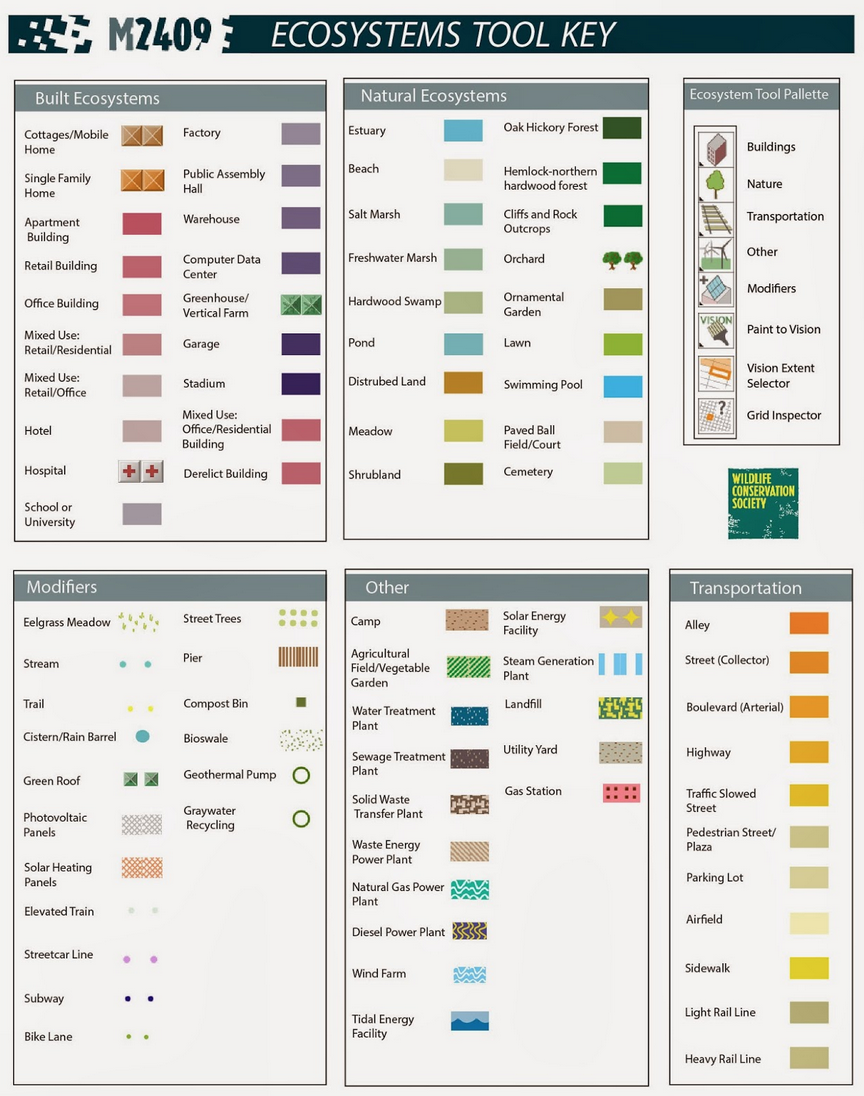
\includegraphics[width=0.9\textwidth]{key.png}
\end{figure}
\end{center}

%----------------------------------------------------------------------------------------

\end{document}